\section{Alaktani
törvényszerűségek}\label{alaktani-tuxf6rvuxe9nyszerux171suxe9gek}

\begin{frame}
A gyakoribb szavak rövidebbek és a nyelvhasználat során gyakrabban /
jobban redukálódnak (Zipf 1936, 1945; Hooper 1976; Phillips 1981, 2006;
Bybee 2000, 2001, 2002; Pierrehumbert 2001; Jurafsky et al.~2001;
Gregory et al.~1999; Bell et al.~2003, 2009; Piantadosi et al.~2011;
Whalen 1991; Gahl 2008; Seyfarth 2014; Arnon \& Cohen Priva 2013; Hay et
al.~2015; Todd et al.~2019; Raymond et al.~2016; Jaeger \& Buz n.d.;
Nettle 1995; Wichmann et al.~2011; Pagel et al.~2007).
\end{frame}

\begin{frame}
A szavak úgy viselkednek, mint más, hozzájuk hasonló szavak (Skousen
1989; Albright \& Hayes 2003; Rácz et al.~2014, 2018, 2020; Krott et
al.~2001; Milin et al.~2009; Dąbrowska 2008; Eddington 2000; Goldsmith
2009; Ernestus \& Baayen 2004; Schryver et al.~2008; Sóskuthy 2013;
Daland et al.~2007; Baayen \& del Prado Martín 2005; Janda et al.~2010;
Lindsay-Smith et al.~2024).
\end{frame}

\section{A jelenség}\label{a-jelensuxe9g}

\begin{frame}{2sg.sbjv}
\protect\phantomsection\label{sg.sbjv}
\begin{itemize}
\tightlist
\item
  várj/várjál
\item
  várd/várjad
\end{itemize}
\end{frame}

\begin{frame}{Hasonlóságok, B}
\protect\phantomsection\label{hasonluxf3suxe1gok-b}
\begin{table}
\centering
\begin{tabular}{llll}
\toprule
\textbf{Tag} & \textbf{Ex} & \textbf{Long 2Sg} & \textbf{Overlap} \\
\midrule
Ind Def 3Sg & \multirow{2}{*}{várja} & \multirow{2}{*}{várjad} & \multirow{2}{*}{ja} \\
Sbjv Def 3Sg & & & \\
Ind Def 3Pl & \multirow{2}{*}{várják} & \multirow{2}{*}{várjál} & \multirow{2}{*}{já} \\
Sbjv Def 3Pl & & & \\
\bottomrule
\end{tabular}
\end{table}
\end{frame}

\begin{frame}{Hasonlóságok, F}
\protect\phantomsection\label{hasonluxf3suxe1gok-f}
\begin{table}
\centering
\begin{tabular}{llll}
\toprule
\textbf{Tag} & \textbf{Ex} & \textbf{Long 2Sg} & \textbf{Overlap} \\
\midrule
Ind Def 3Sg & kéri & \multirow{2}{*}{kérjed} & $\emptyset{}$ \\
Sbjv Def 3Sg & kérje & & je \\
Ind Def 3Pl & kérik & \multirow{2}{*}{kérjél} & $\emptyset{}$ \\
Sbjv Def 3Pl & kérjék & & já \\
\bottomrule
\end{tabular}
\end{table}
\end{frame}

\section{Kérdések}\label{kuxe9rduxe9sek}

\begin{frame}{Kérdések}
Mitől lesz valami inkább akármizz / akármizzél?

\begin{enumerate}
\tightlist
\item
  Számít a tő hossza vagy gyakorisága?
\item
  Számít az alaktani előfeszítés? (várja/várjad de kéri/kérjed)
\item
  Számít a határozottság? (várjál/várjad)
\end{enumerate}
\end{frame}

\section{Válaszok}\label{vuxe1laszok}

\begin{frame}{Válaszok}
\begin{itemize}
\tightlist
\item
  Korpusz
\item
  Kísérlet
\end{itemize}
\end{frame}

\begin{frame}{Korpusz}
\protect\phantomsection\label{korpusz}
\begin{itemize}
\tightlist
\item
  Magyar Webkorpusz 2 gyakorisági lista (Nemeskey 2022, Rácz 2026)
\item
  igék, amelyeknek van 2sg.sbjv alakjuk, és

  \begin{itemize}
  \tightlist
  \item
    nem -t/-ik végűek
  \item
    nem tesz/vesz/hisz/visz/eszik/iszik
  \item
    legalább tíz előfordulás összesen (nem csak 2sg.sbjv)
  \end{itemize}
\item
  1480 igető
\end{itemize}
\end{frame}

\begin{frame}{Módszer}
\protect\phantomsection\label{muxf3dszer}
\begin{itemize}
\tightlist
\item
  outcome: hosszú / rövid 2sg.sbjv alakok aránya
\item
  prediktorok:

  \begin{itemize}
  \tightlist
  \item
    sbjv def/indef
  \item
    tő egy v többszótagos
  \item
    tő log lemmagyakoriság
  \item
    tő elöl/hátulképzett
  \item
    tő 3sg def/indef arány
  \end{itemize}
\item
  logisztikus OLRE GLMM megfigyelés- és lemma-RI-el
\item
  két motivált interakció: tő 3sg def/indef arány * sbjv def/indef +
  arány * stem\_harmony + tő egy v többszótagos + tő log lemmagyakoriság
\end{itemize}
\end{frame}

\begin{frame}{Eredmények}
\protect\phantomsection\label{eredmuxe9nyek}
\begin{block}{Eloszlások}
\protect\phantomsection\label{eloszluxe1sok}
\begin{figure}
\centering
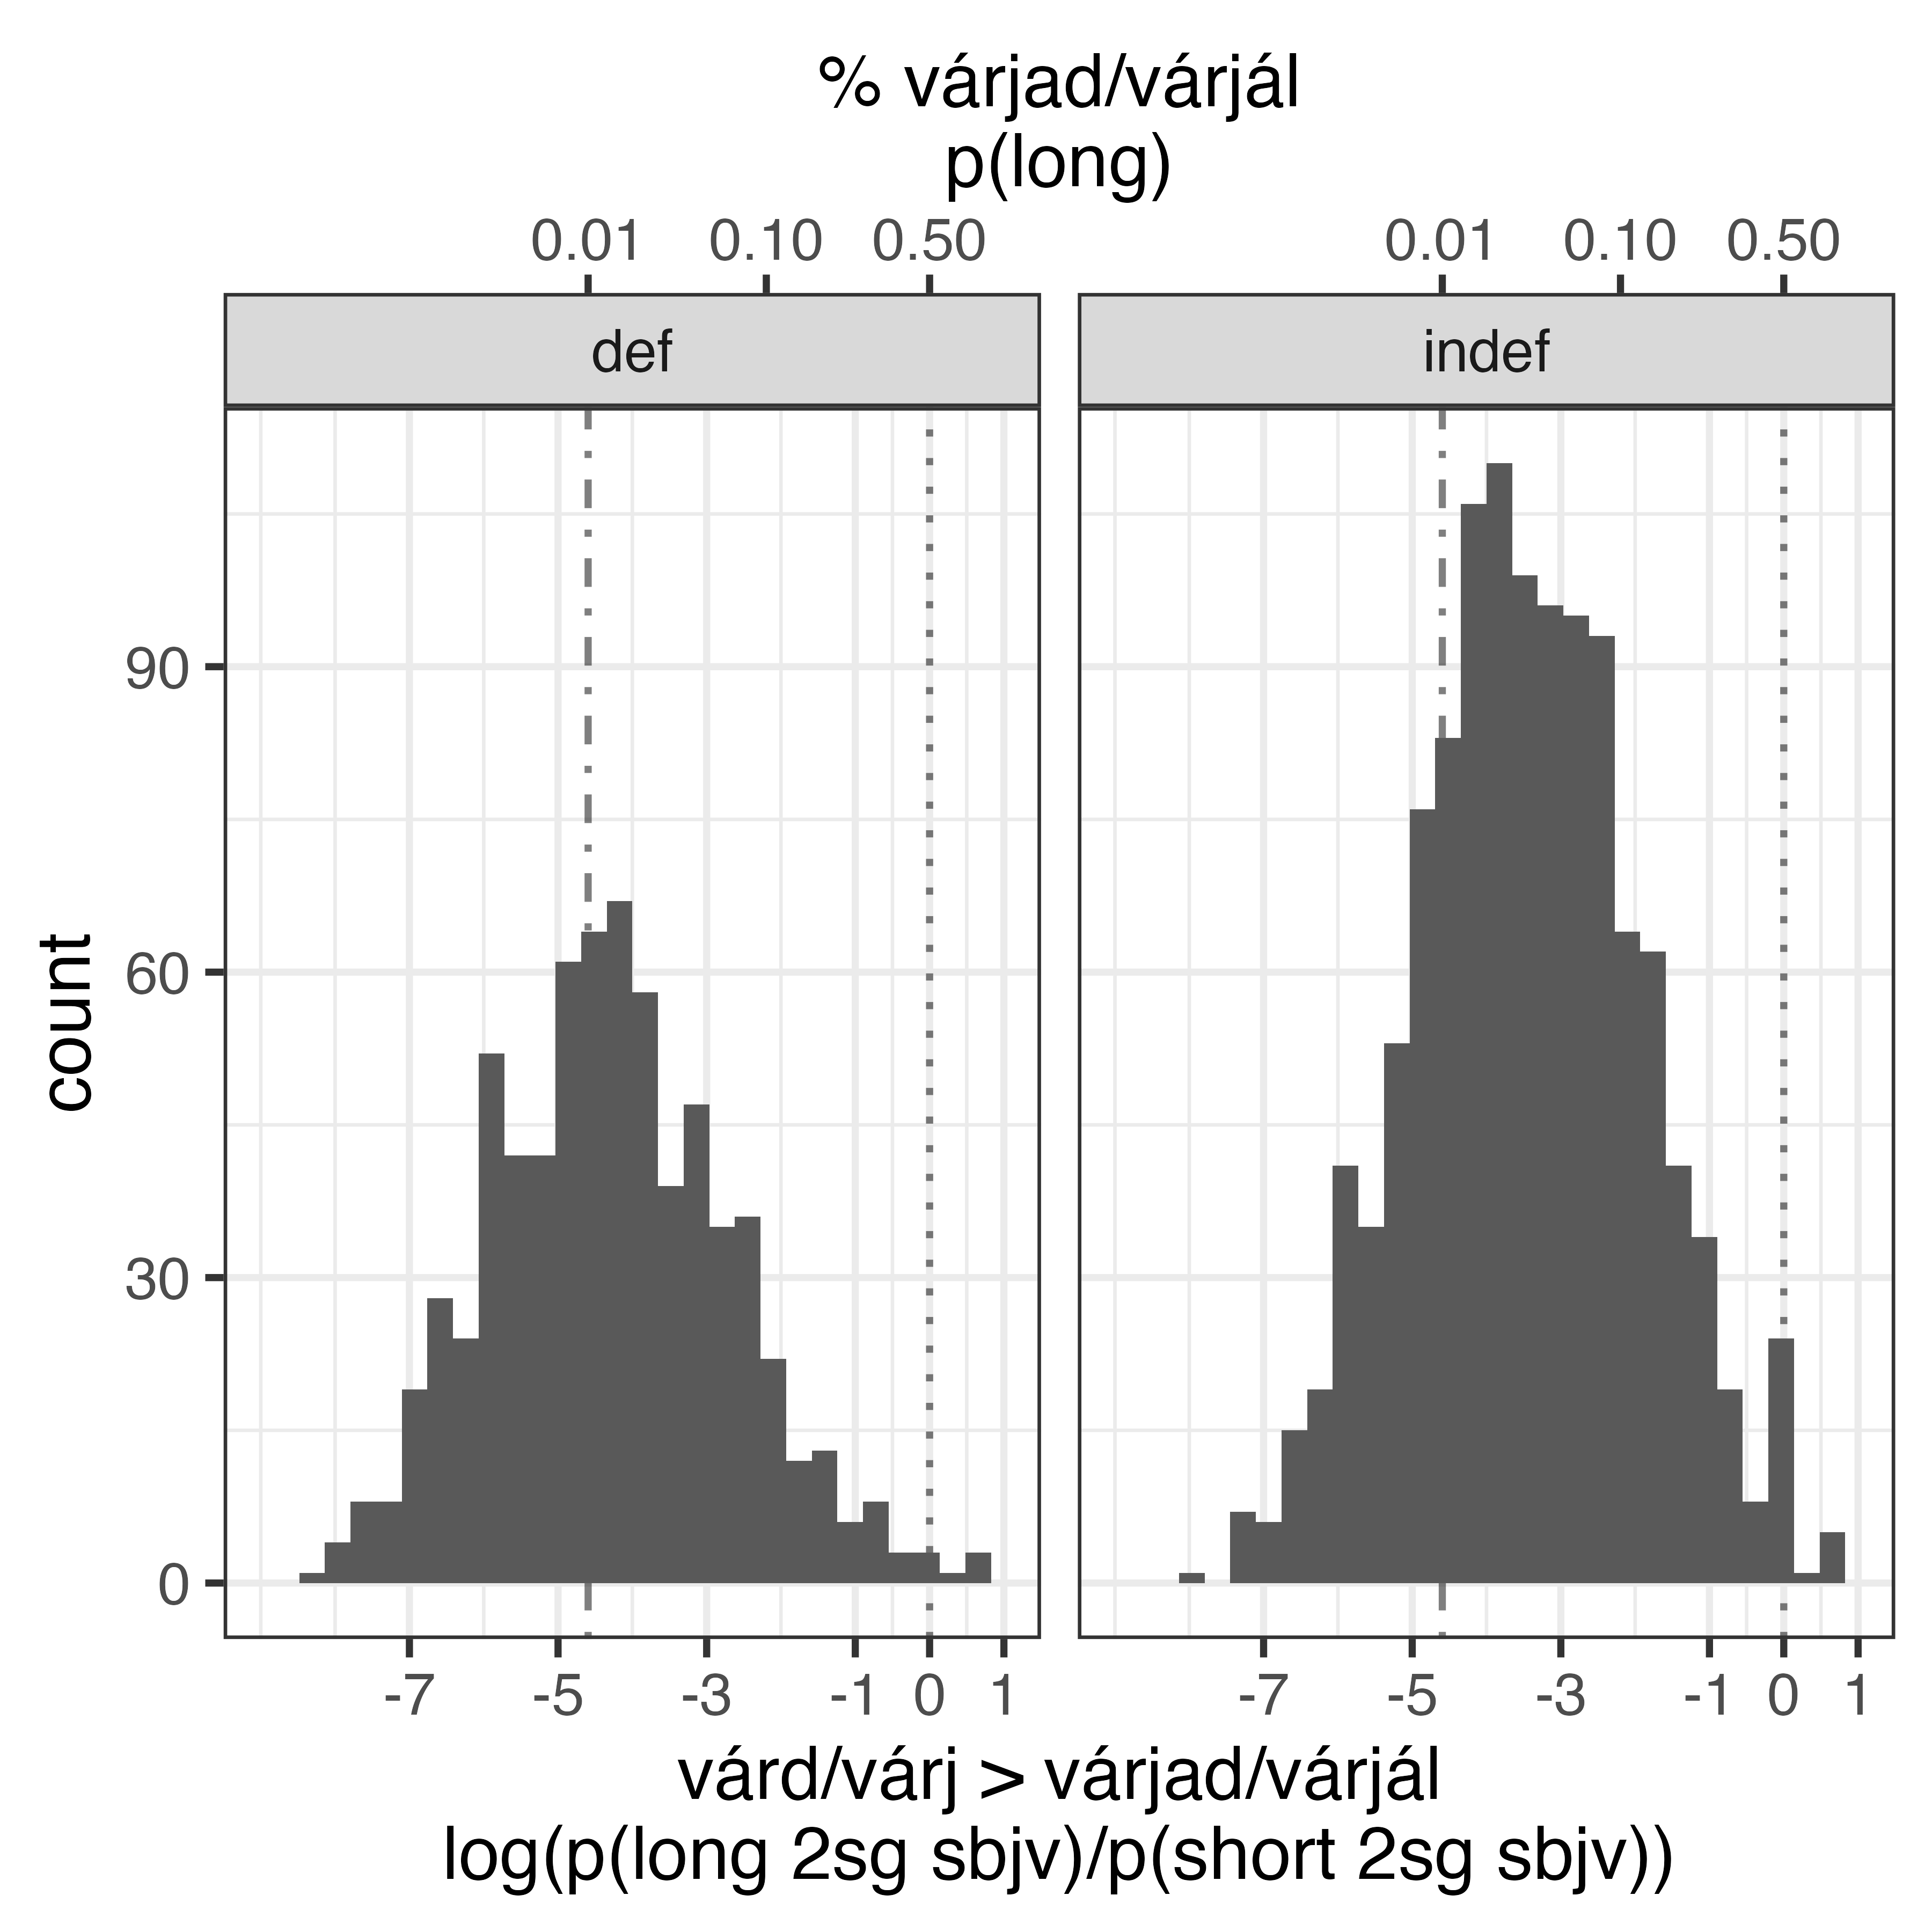
\includegraphics[width=0.85\textwidth]{viz/adjal_manyek_0.png}
\end{figure}
\end{block}

\begin{block}{Gyakoriság}
\protect\phantomsection\label{gyakorisuxe1g}
\begin{figure}
\centering
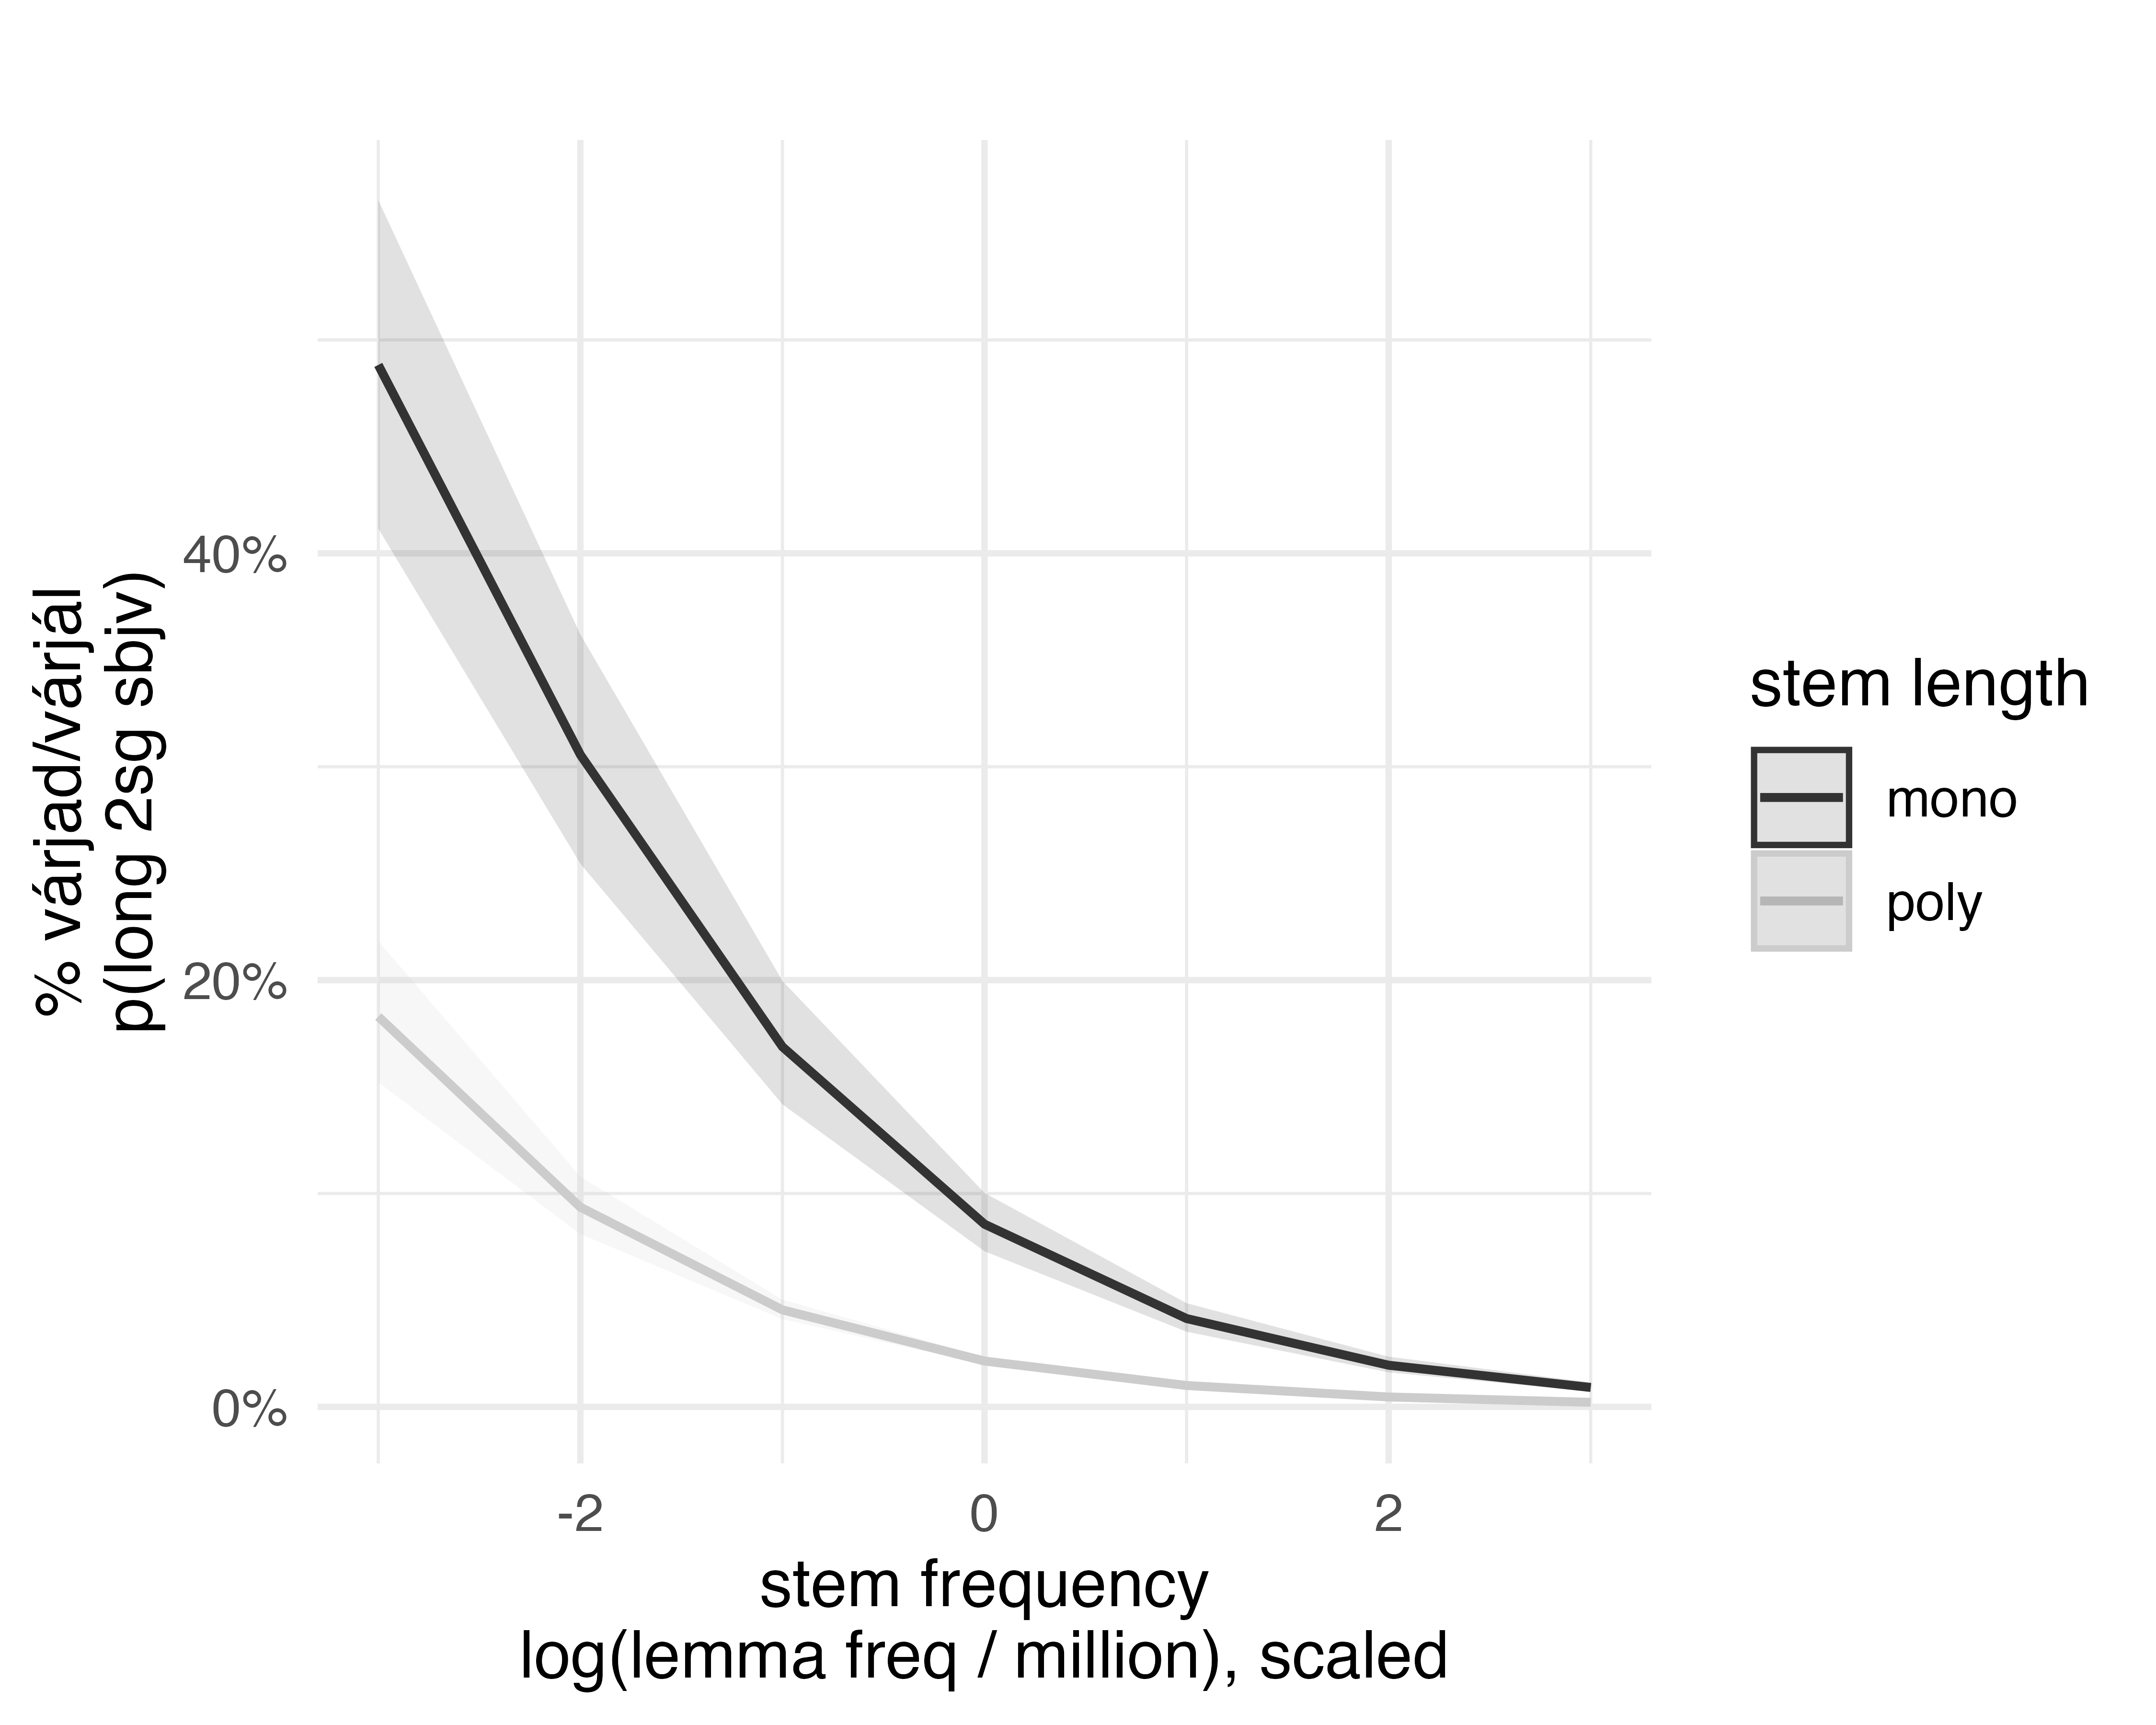
\includegraphics[width=0.85\textwidth]{viz/adjal_manyek_1.png}
\end{figure}
\end{block}

\begin{block}{Hasonlóság}
\protect\phantomsection\label{hasonluxf3suxe1g}
\begin{figure}
\centering
\includegraphics[width=0.85\textwidth]{viz/adjal_manyek_2.png}
\end{figure}
\end{block}

\begin{block}{Határozottság}
\protect\phantomsection\label{hatuxe1rozottsuxe1g}
\begin{figure}
\centering
\includegraphics[width=0.85\textwidth]{viz/adjal_manyek_3.png}
\end{figure}
\end{block}
\end{frame}

\begin{frame}{Összefoglalva}
\protect\phantomsection\label{uxf6sszefoglalva}
\begin{itemize}
\tightlist
\item
  a gyakoribb igetövek jobban szeretik a rövidebb kötőmódot
\item
  az egyszótagos / többszótagos igetövek eltérnek egymástól
\item
  az alaki hasonlóság mindegy: a teljesen máshogyan kinéző elöl- és
  hátulképzett tövek viselkedésében nem látunk különbséget
\item
  a def / indef paradigma támogatottsága számít: ha eleve sok a def
  alak, ezek rövidebbek lesznek, és vice versa
\end{itemize}
\end{frame}

\begin{frame}{Összefoglalva}
\protect\phantomsection\label{uxf6sszefoglalva-1}
\begin{enumerate}
\tightlist
\item
  Számít a tő hossza vagy gyakorisága!
\item
  Nem számít az alaktani előfeszítés! (várja/várjad de kéri/kérjed)
\item
  Számít a határozottság! (várjál/várjad)
\end{enumerate}
\end{frame}

\section{Kísérlet}\label{kuxedsuxe9rlet}

\begin{frame}{Adatgyűjtés}
\protect\phantomsection\label{adatgyux171jtuxe9s}
\begin{itemize}
\tightlist
\item
  adj / adjál? nem jó, mert az embereknek vannak stilisztikai
  beakadásaik
\item
  legyen előfeszítés, mert az nem annyira tudatos
\end{itemize}
\end{frame}

\begin{frame}{Előfeszítés / priming}
\protect\phantomsection\label{elux151feszuxedtuxe9s-priming}
\begin{itemize}
\tightlist
\item
  előfeszítő inger
\item
  célinger, amit elfogadsz vagy elutasítasz
\item
  vannak kamu célingerek, hogy lássuk, odafigyelsz
\item
  a valódi célingerekre adott reakcióidőt mérjük
\end{itemize}
\end{frame}

\begin{frame}
{\def\LTcaptype{none} % do not increment counter
\begin{longtable}[]{@{}lllll@{}}
\toprule\noalign{}
prime & target & alaktan & hangtan & \\
\midrule\noalign{}
\endhead
várjad & várd & ✓ & ❌ & competition \\
várjad & várja & ❌ & ✓ & similarity \\
kérjed & kérd & ✓ & ❌ & competition \\
kérjed & kéri & ❌ & ❌ & pffff \\
\bottomrule\noalign{}
\end{longtable}
}
\end{frame}

\begin{frame}
{\def\LTcaptype{none} % do not increment counter
\begin{longtable}[]{@{}
  >{\raggedright\arraybackslash}p{(\linewidth - 12\tabcolsep) * \real{0.0597}}
  >{\raggedright\arraybackslash}p{(\linewidth - 12\tabcolsep) * \real{0.1940}}
  >{\raggedright\arraybackslash}p{(\linewidth - 12\tabcolsep) * \real{0.0746}}
  >{\raggedright\arraybackslash}p{(\linewidth - 12\tabcolsep) * \real{0.1940}}
  >{\raggedright\arraybackslash}p{(\linewidth - 12\tabcolsep) * \real{0.0746}}
  >{\raggedright\arraybackslash}p{(\linewidth - 12\tabcolsep) * \real{0.2090}}
  >{\raggedright\arraybackslash}p{(\linewidth - 12\tabcolsep) * \real{0.1940}}@{}}
\toprule\noalign{}
\begin{minipage}[b]{\linewidth}\raggedright
H0
\end{minipage} & \begin{minipage}[b]{\linewidth}\raggedright
várd-várjad
\end{minipage} & \begin{minipage}[b]{\linewidth}\raggedright
=
\end{minipage} & \begin{minipage}[b]{\linewidth}\raggedright
kéri-kérjed
\end{minipage} & \begin{minipage}[b]{\linewidth}\raggedright
=
\end{minipage} & \begin{minipage}[b]{\linewidth}\raggedright
várja-várjad
\end{minipage} & \begin{minipage}[b]{\linewidth}\raggedright
semmi
\end{minipage} \\
\midrule\noalign{}
\endhead
H1 & várd-várjad & \textgreater{} & kéri-kérjed & = & várja-várjad &
csak morf \\
H2 & várd-várjad & = & kéri-kérjed & \textgreater{} & várja-várjad &
csak fon \\
H3 & várd-várjad & \textgreater{} & kéri-kérjed & \textgreater{} &
várja-várjad & fon és morf \\
\bottomrule\noalign{}
\end{longtable}
}
\end{frame}
